\chapter{PARA/LLAX} 
\label{sec:parallax}
\lstset{style=6502Style}

\vspace{-2.0cm}
\begin{figure}[H]
    \begin{adjustbox}{width=13.3cm,left}
      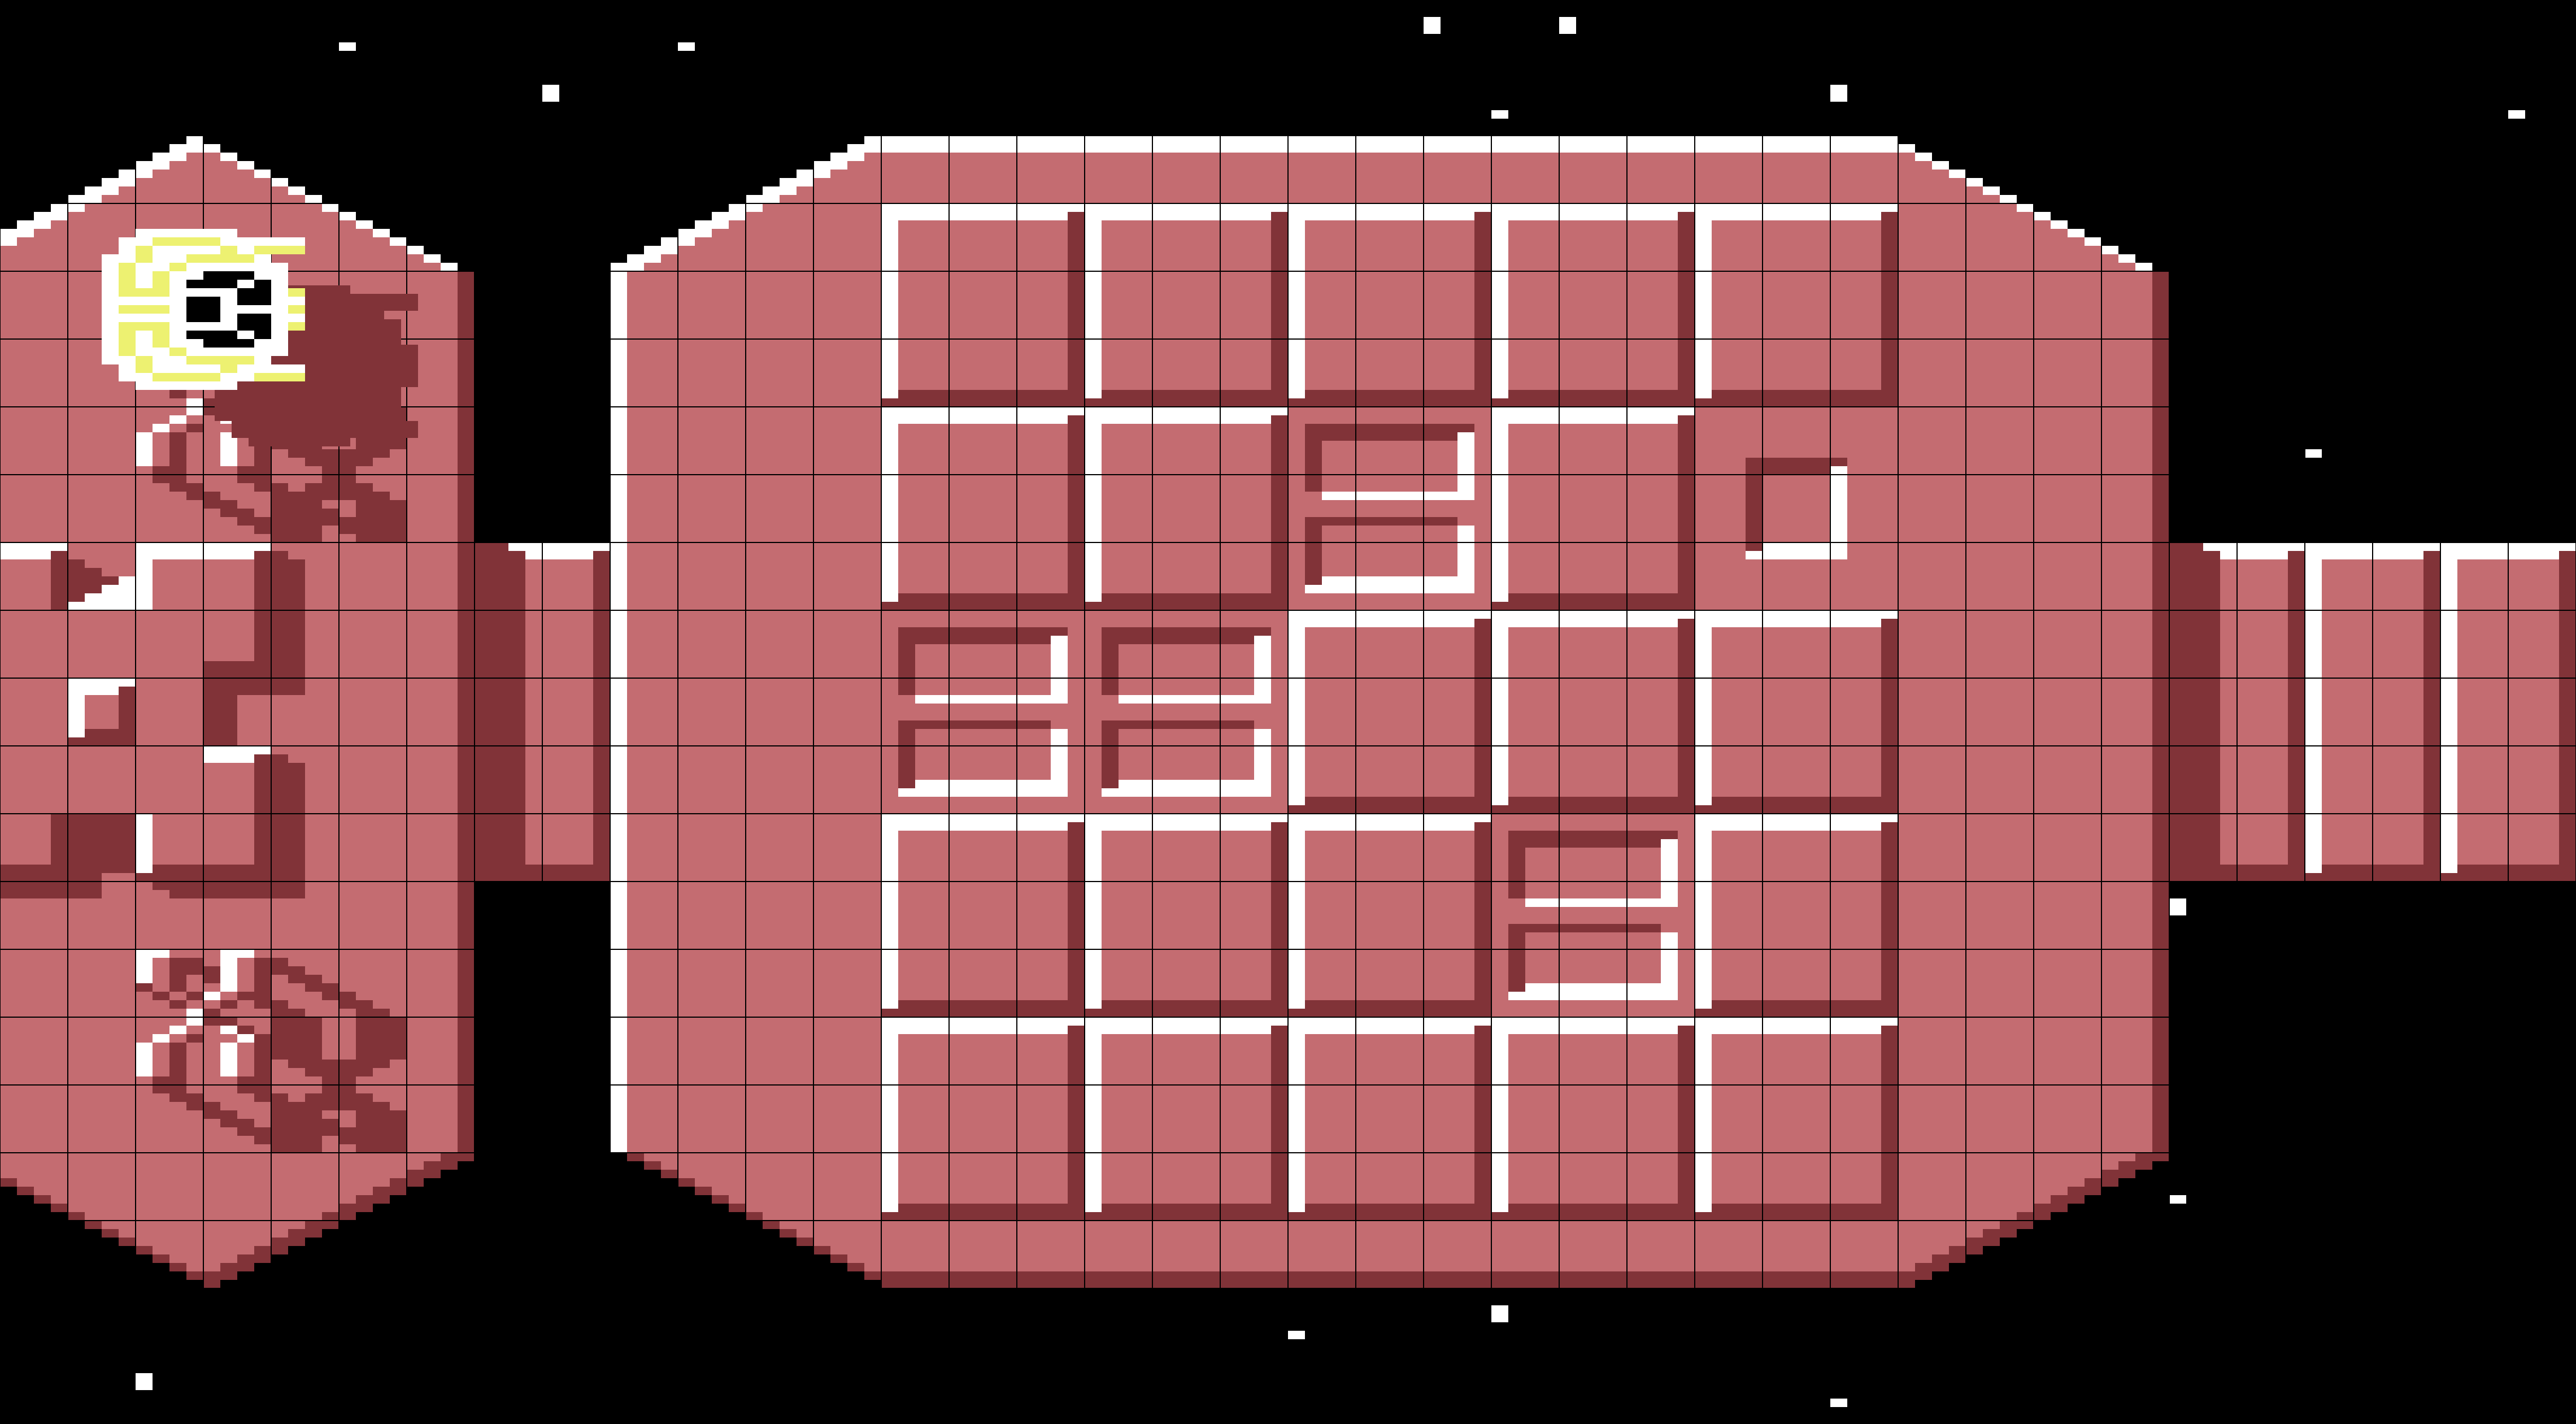
\includegraphics{src/starfield/dreadnought_with_stars.png}%
    \end{adjustbox}
\end{figure}
\vspace{-0.4cm}

Behind the dreadnought lies a sparse field of stars. As we zip along the surface they
remain completely still, creating an impression of parallax: the stars remain static because they are so distant. No
matter how fast we move, they are so far away that from our perspective they will never move.

At first this might not seem a difficult effect to achieve, but it does require some thinking about. As the
surface of the dreadnought scrolls across the screen we must find some way of ensuring that the stars do not
scroll along with it. In addition to that we must ensure that the stars behind the dreadnought peek through
the gaps between sections when they roll into view. It is this last feature that is arguably vital to completing
the illusion of a distant starfield.

Let's start by looking at what we will use to draw the stars themselves. Careful inspection reveals there are two
sizes in use: a small star (\icode{\$42}) and a big star (\icode{\$43}). Each type is just two pixels wide and 
defined at the far left edge of the character specification it occupies. In order to minimize the appearance of our
stars appearing in neat rows when drawn on the same line we also place them at slightly different vertical positions within the specification.

\begin{figure}[H]
    \centering
    \begin{adjustbox}{center}
      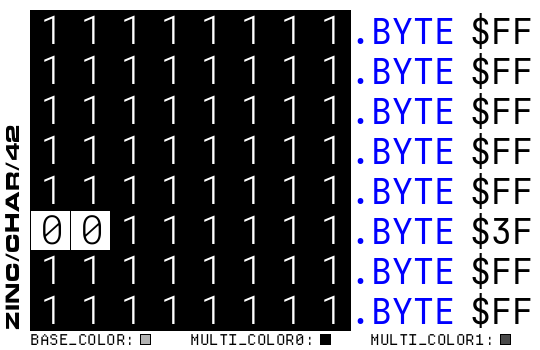
\includegraphics[width=6.50cm]{src/character_set_diagrams/1_42.png}%
      \hspace{0.2cm}
      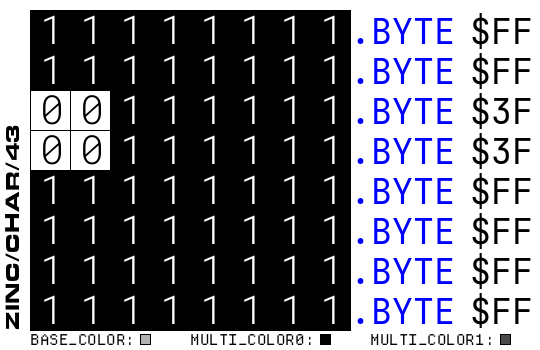
\includegraphics[width=6.50cm]{src/character_set_diagrams/1_43.png}%
    \end{adjustbox}
\end{figure}
\vspace{-0.4cm}

At the start of each level we will generate a new randomly positioned field of stars. We break this exercise up into
three parts: the vacant area below the dreadnought, the empty space above it, and finally the area normally covered by the dreadnought.

Here we accomplish the first part, we sprinkle a dusting of stars across the bottom two lines of the screen.
\begin{lstlisting}
GenerateStarfield
  ; Make ramLoPtr/ramHiPtr refer to the bottom line of the screen.
  LDX #<SCREEN_RAM + $00A0 ; Load the low byte of the address to X.
  LDY #>SCREEN_RAM + $00A0 ; Load the high byte of the address to Y.
  STX ramLoPtr             ; Store as the low byte pointer.
  STY ramHiPtr             ; Store as the high byte pointer.

  LDA #$30                 ; Load 48 to A.
  STA dataIndex            ; Store it as our index into random data.
  JSR WriteARowOfStars     ; Write a row of stars to the line.

  ; Move our pointer to point to the line above.
  LDA ramLoPtr             ; Load ramLoPtr to A.
  ADC #$28                 ; Increment by 40.
  STA ramLoPtr             ; Store updated value in ramLoPtr.
  JSR WriteARowOfStars     ; Write a row of stars to the line.
\end{lstlisting}

This is an example of what the result looks like. The positioning is random, so can often be uneven or even outright clumpy.
\begin{figure}[H]
    \begin{adjustbox}{width=13.3cm,left}
      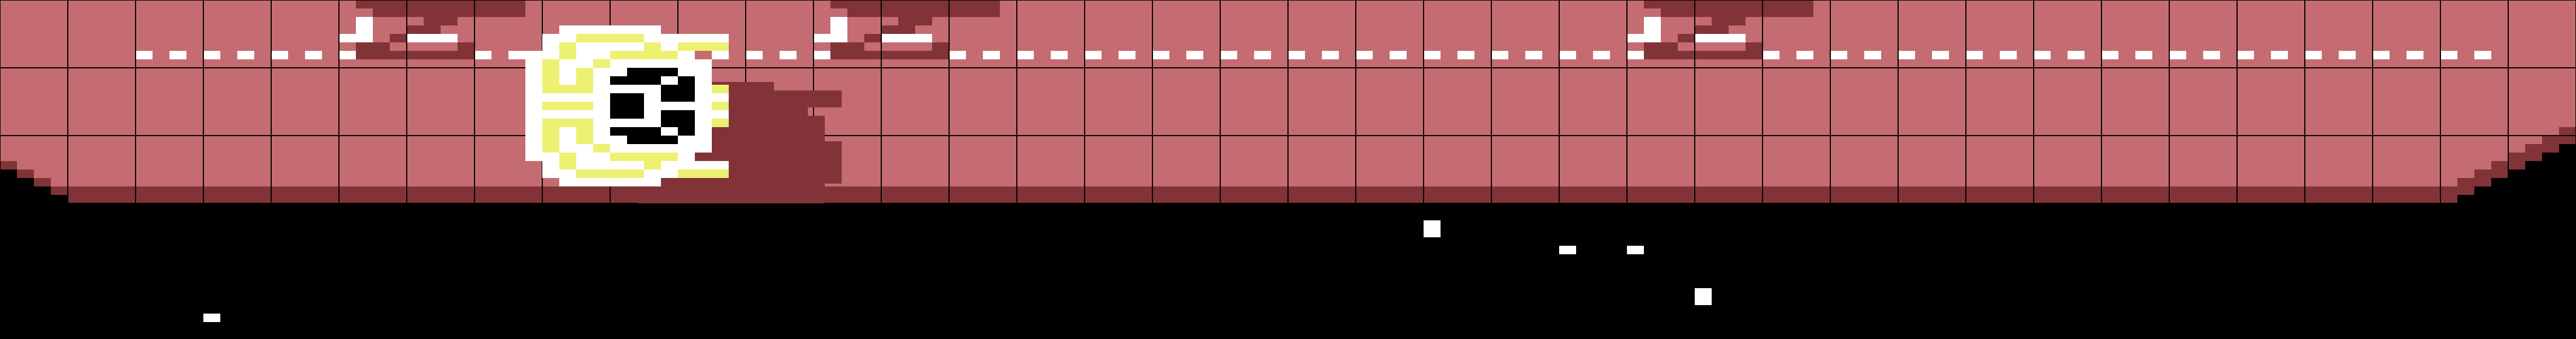
\includegraphics{src/starfield/dreadnought_with_stars_bottom.png}%
    \end{adjustbox}
\end{figure}
\vspace{-0.4cm}

In the routine above it is the subroutine \icode{WriteARowOfStars} that is doing this heavy lifting, so that is where we need
to look to get an idea of how the distribution of the stars on a line is achieved in practice. What we find is that
for each character in the line we pluck a value from a pool of random values stored in the \icode{randomData} array. If the value
we retrieve is less than 240 (\icode{\$F0}) we draw a blank space. If it is less than 248 (\icode{\$F8}) we draw a
small star (\icode{\$42}). Otherwise we draw a big star (\icode{\$43}).  

\begin{lstlisting}
WriteARowOfStars
  LDY #38            ; Load 38 to Y, i.e. write 38 characters.
WriteStarsLoop
  LDX dataIndex      ; Load our index to X.
  LDA randomData,X   ; Use it to fetch a random number.
  INC dataIndex      ; Increment our index.
  TAX                ; Transfer our random number to X.
  LDA #$20           ; Load 'space' to A.
  CPX #$F0           ; Compare our random number with 240.
  BCC WriteValue     ; If it's less than write a space.
  LDA #$42           ; Load the small star to A.
  CPX #$F8           ; Compare our random number with 248.
  BCS WriteValue     ; If it's less, then use the small star. 
  ADC #$01           ; Otherwise add 1 to use the large star ($43).
WriteValue
  STA (ramLoPtr),Y   ; Write the selected value to screen.
  DEY                ; Move to the next position in the row.
  BPL WriteStarsLoop ; Keep going until Y reaches zero.
  RTS
\end{lstlisting}

So the sparsity of stars is achieved by drawing one at any given position with an approximate probability of 1 in 20. Our source of random data (which is ultimately
the C64's built-in random number generator) gives us a number between 0 and 255 and we only draw a star when that number is
between 240 and 255, otherwise we draw black space. 

In practice this means that for the most part we will likely as not draw at least two stars on each line. There will be occasions when we
draw more than that and as we can see in our examples so far there is nothing in our process to prevent stars clumping together. Worse,
the randomness inherent to the procedure means that there will be even be some small number of instances where we draw just one or even zero stars on a line.

This is not what we observe in most cases though - the odds mean that for the most part we will almost always get somewhere between two and
four stars on each row. We can see this when we proceed to the second part of our starfield generation procedure. Here we draw another two rows
of stars at the top of the screen by adjusting the our starting point in \icode{ramLoPtr} and \icode{ramHiPtr}:

\begin{lstlisting}
  ; Make ramLoPtr/ramHiPtr refer to the bottom line of the screen.
  LDX #<SCREEN_RAM + $0398 ; Load the low byte of the address to X.
  LDY #>SCREEN_RAM + $0398 ; Load the high byte of the address to Y.
  STX ramLoPtr             ; Store as the low byte pointer.
  STY ramHiPtr             ; Store as the high byte pointer.
  JSR WriteARowOfStars     ; Write a row of stars to the line.

  ; Move our pointer to point to the line above.
  LDA ramLoPtr             ; Load ramLoPtr to A.
  ADC #$28                 ; Increment by 40.
  STA ramLoPtr             ; Store updated value in ramLoPtr.
  JSR WriteARowOfStars     ; Write a row of stars to the line.
\end{lstlisting}

In this example we get two stars on the first row and four on the second.
\begin{figure}[H]
    \begin{adjustbox}{width=13.3cm,left}
      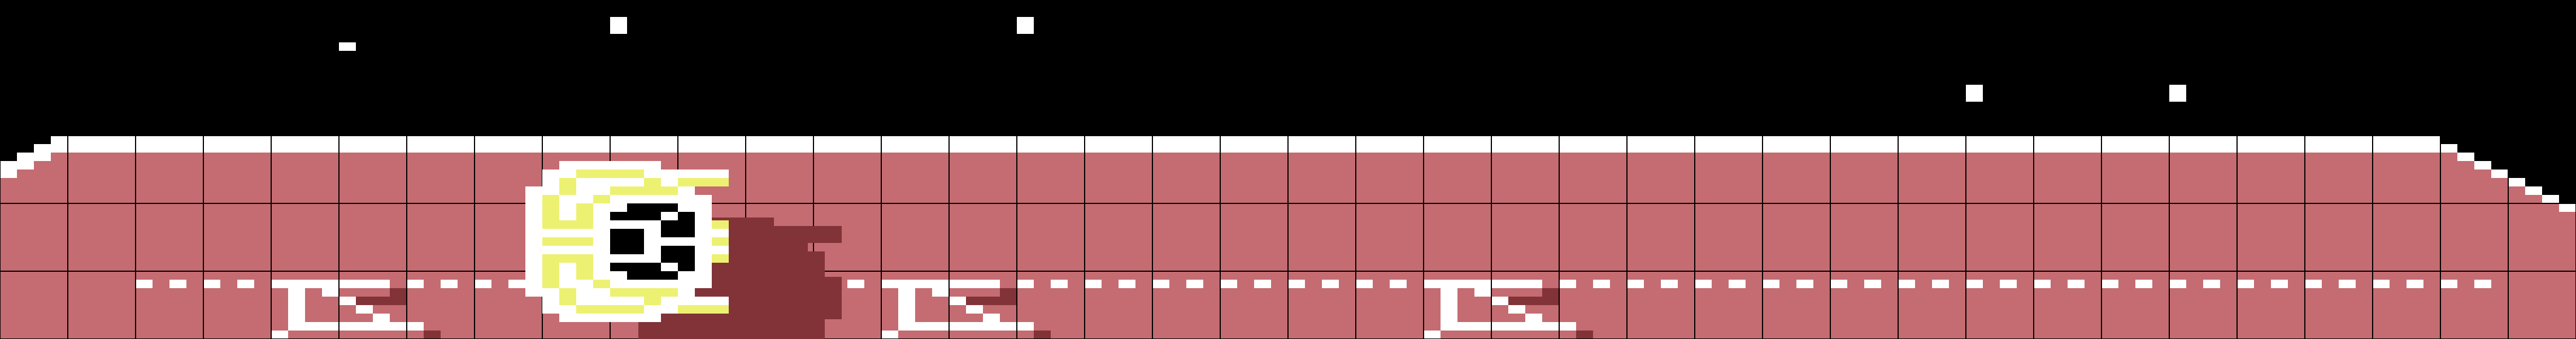
\includegraphics{src/starfield/dreadnought_with_stars_top.png}%
    \end{adjustbox}
\end{figure}
\vspace{-0.4cm}

Our third and final step is to come up with a general background of stars that will poke out between the gaps
in the dreadnought as we travel across it. To do that we will pre-populate a list of 16 randomly distributed large
and small stars. When the time comes to display these background stars we will go through the list and determine
which of them are visible and can be displayed. In the routine on the opposite page we generate this list and store
its information in 3 separate arrays. The first two arrays are \icode{starDataLoPtrArray} and \icode{starDataHiPtrArray}.
Together these give us the location of each star on the screen. The third array is \icode{starsBehindDreadnought}. This
tells us whether each star is large or small. Two examples of the kind of distribution this routine gives are illustrated below.

\begin{figure}[H]
    \centering
    \begin{adjustbox}{center}
      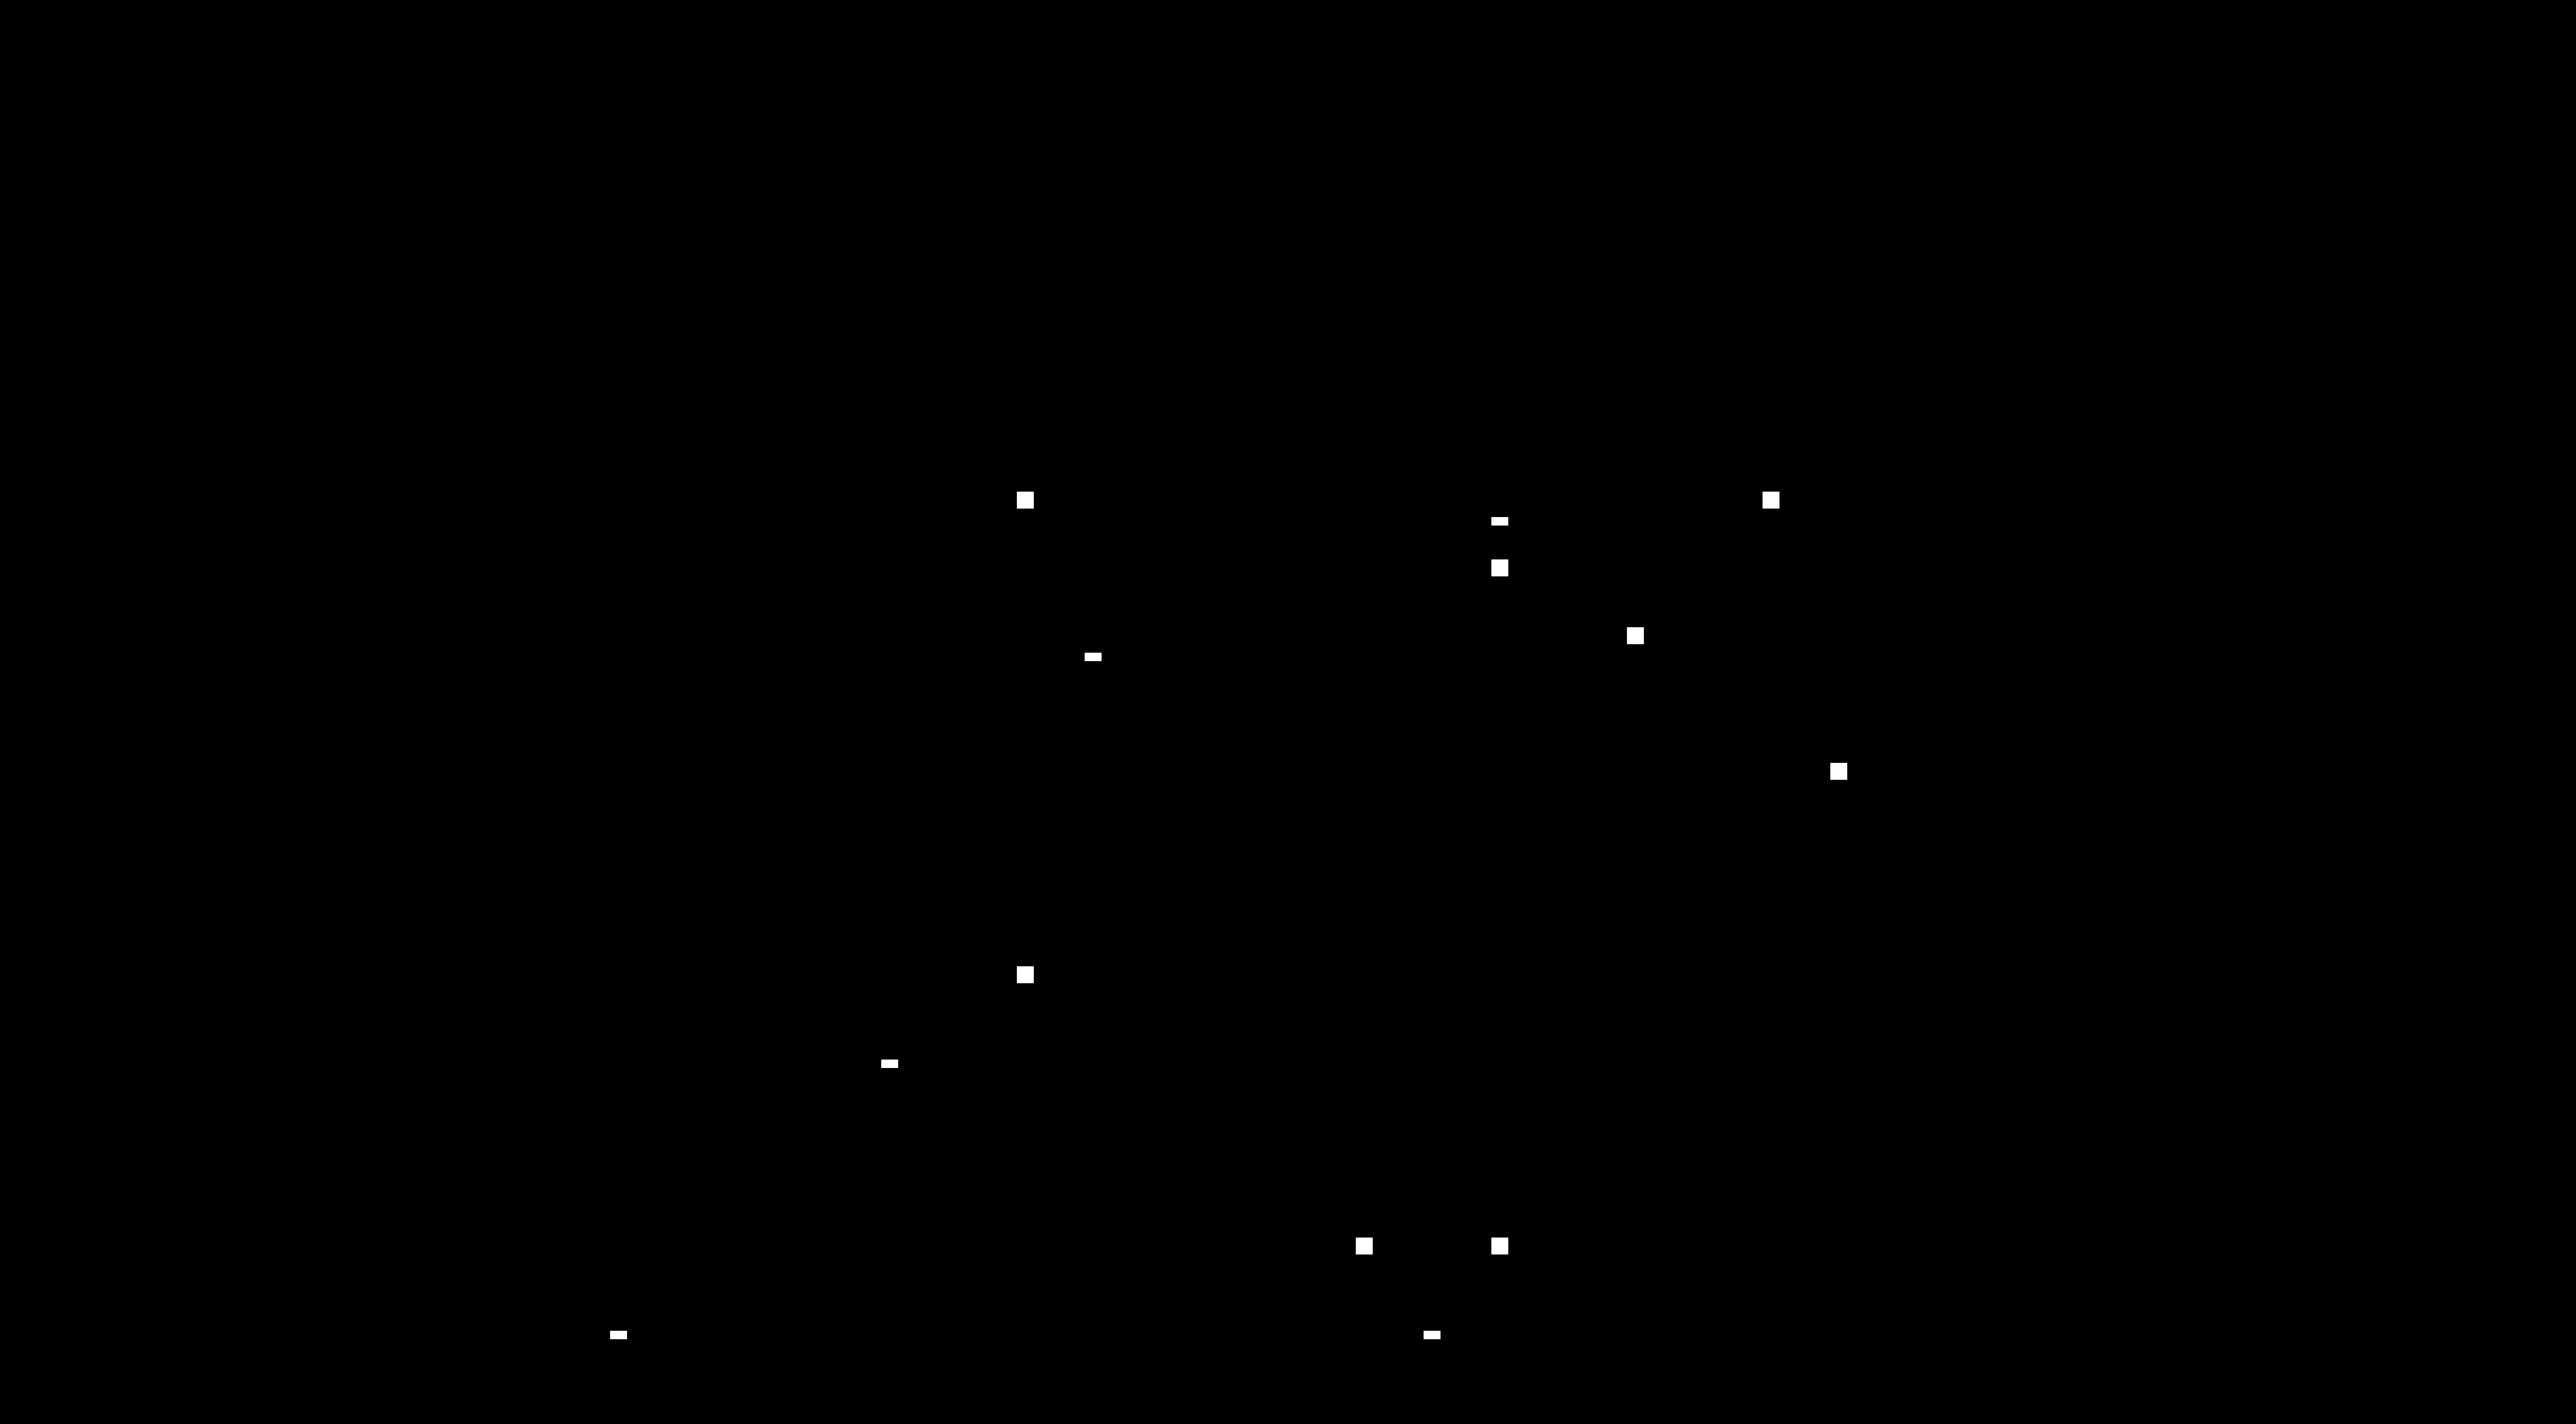
\includegraphics[width=6.50cm]{src/starfield/background_stars.png}%
      \hspace{0.2cm}
      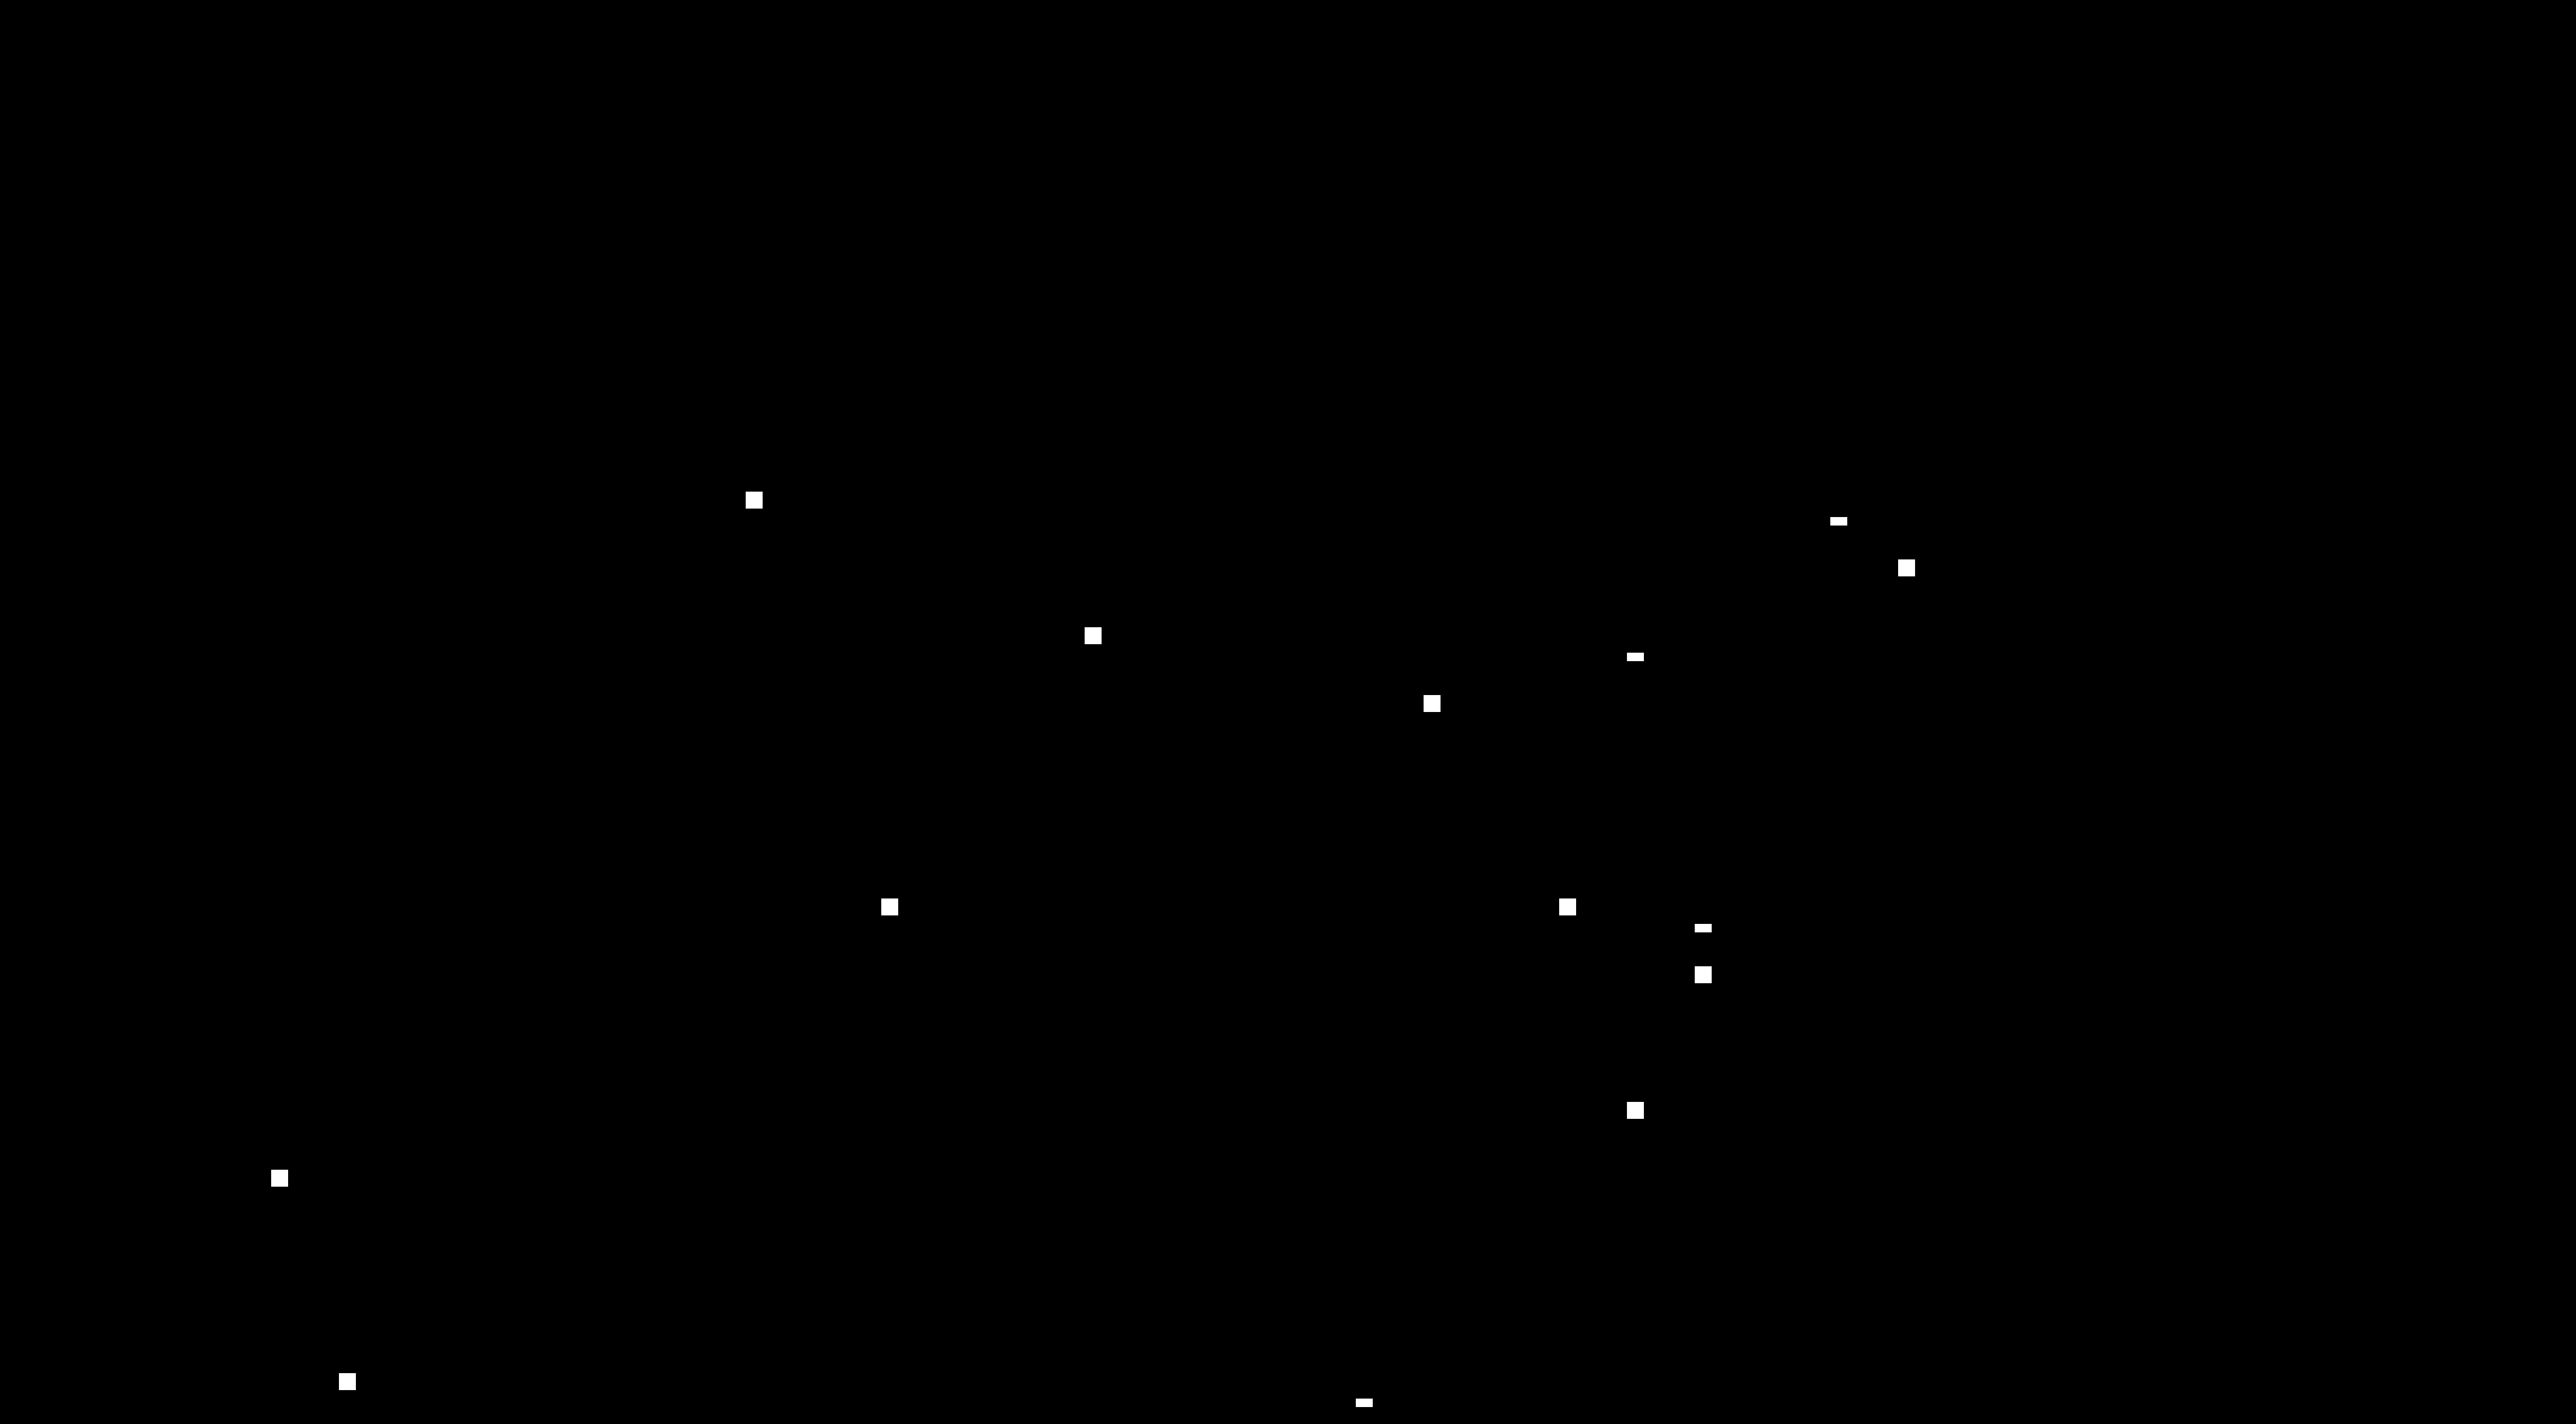
\includegraphics[width=6.50cm]{src/starfield/background_stars_2.png}%
    \end{adjustbox}
\end{figure}
\vspace{-0.4cm}


\clearpage
\begin{lstlisting}
GenerateStarData
  LDY #$0F           ; We are going to add 16 stars in total.
  LDA #$00           ; Load zero the A register.
  STA dataIndex      ; And store it in dataIndex.

AddStarsLoop
  ; Get a random number between 7 and 22 and store it in X.
  LDX dataIndex      ; Load our index to X.
  LDA randomData,X   ; Use it to fetch a random number.
  INC dataIndex      ; Increment our index.
  AND #$0F           ; Clamp random numbeer between 0 and 15.
  ADC #$07           ; Add 7 to it.
  TAX                ; Store our random number in X.

  ; Use our random number (in X) to select a line on the screen.
  LDA screenLineHiPtrArray,X
  STA starDataHiPtrArray,Y
  LDA screenLineLoPtrArray,X
  STA starDataLoPtrArray,Y
  LDA colorLineHiPtrArray,X
  STA currentColorLineHiPtrArray,Y

  ; Get a random number between 4 and 31 and store it in X.
  LDX dataIndex      ; Load our index to X.
  LDA randomData,X   ; Use it to fetch a random number.
  INC dataIndex      ; Increment our index.
  AND #$1F           ; Clamp random number between 0 and 31.
  CMP #$14           ; Compare it to 20.
  BCC SkipAdding4    ; If it's less than 20..
  ADC #$04           ; .. then add 4.
SkipAdding4                
  TAX                ; Store our random number in X.

  ; Use the random number (in X) to select a position on the line.
  TXA                ; Store our random number in A.
  ADC starDataLoPtrArray,Y ; Add it to give a position on the line.
  STA starDataLoPtrArray,Y ; Store the new position on the line.

  ; Get a random number between $42 and $43 and store it in X.
  LDX dataIndex      ; Load our index to X.
  LDA randomData,X   ; Use it to fetch a random number.
  INC dataIndex      ; Increment our index.
  AND #$01           ; Clamp random number between 0 and 1.
  ADC #$42           ; Add $42, so result will be either $42 or $43.

  ; Use this random number (in X) to select a star type.
  STA starsBehindDreadnought,Y  ; Store the selected star.

  DEY                ; Move to the next position in the row.
  BPL AddStarsLoop   ; Keep going until Y reaches zero.

  RTS                ; Return when we're done.
\end{lstlisting}
\clearpage
When the time comes to draw the screen, we don't add all of these stars of course.
Just the ones whose position co-incides with a chink in the dreadnought's surface or 
with the gaps between sections of its deck. In the example below, we can see a star
through two of the transoms as well as one between the couplings on the left. All the
others have been ignored as they would overwrite the deck itself.
Here we see the routine responsible for reading through the list of stars and deciding
which ones to draw. It is as straightforward as discarding any that would not be drawn
on a piece of inky black space.

\begin{lstlisting}
AddStarsBehindDreadnought
  LDX numberOfStarsToAdd    ; Load number of stars to add to X.
AddStarsLoop
  LDA starDataHiPtrArray,X  ; Get the high byte address of the star.
  STA screenHiPtr           ; Store it.
  LDA starDataLoPtrArray,X  ; Get the low byte address of the star.
  STA screenLoPtr           ; Store it.
  LDY #$00                  ; Store 0 in Y.
  LDA (screenLoPtr),Y       ; Get current character at star's position.
  CMP #$20                  ; Is it inky blank space?
  BNE SkipStar              ; If not, skip it.
  ; If it is a gap in the dreadnought, we can draw our star.
  LDA starsBehindDreadnought,X ; Get the type of star. 
  STA (screenLoPtr),Y       ; Draw it to the location.
SkipStar
  DEX                       ; Go the next star.
  BPL AddStarsLoop          ; Keep going until X reaches zero.
\end{lstlisting}

\begin{figure}[H]
    \begin{adjustbox}{width=13.3cm,left}
      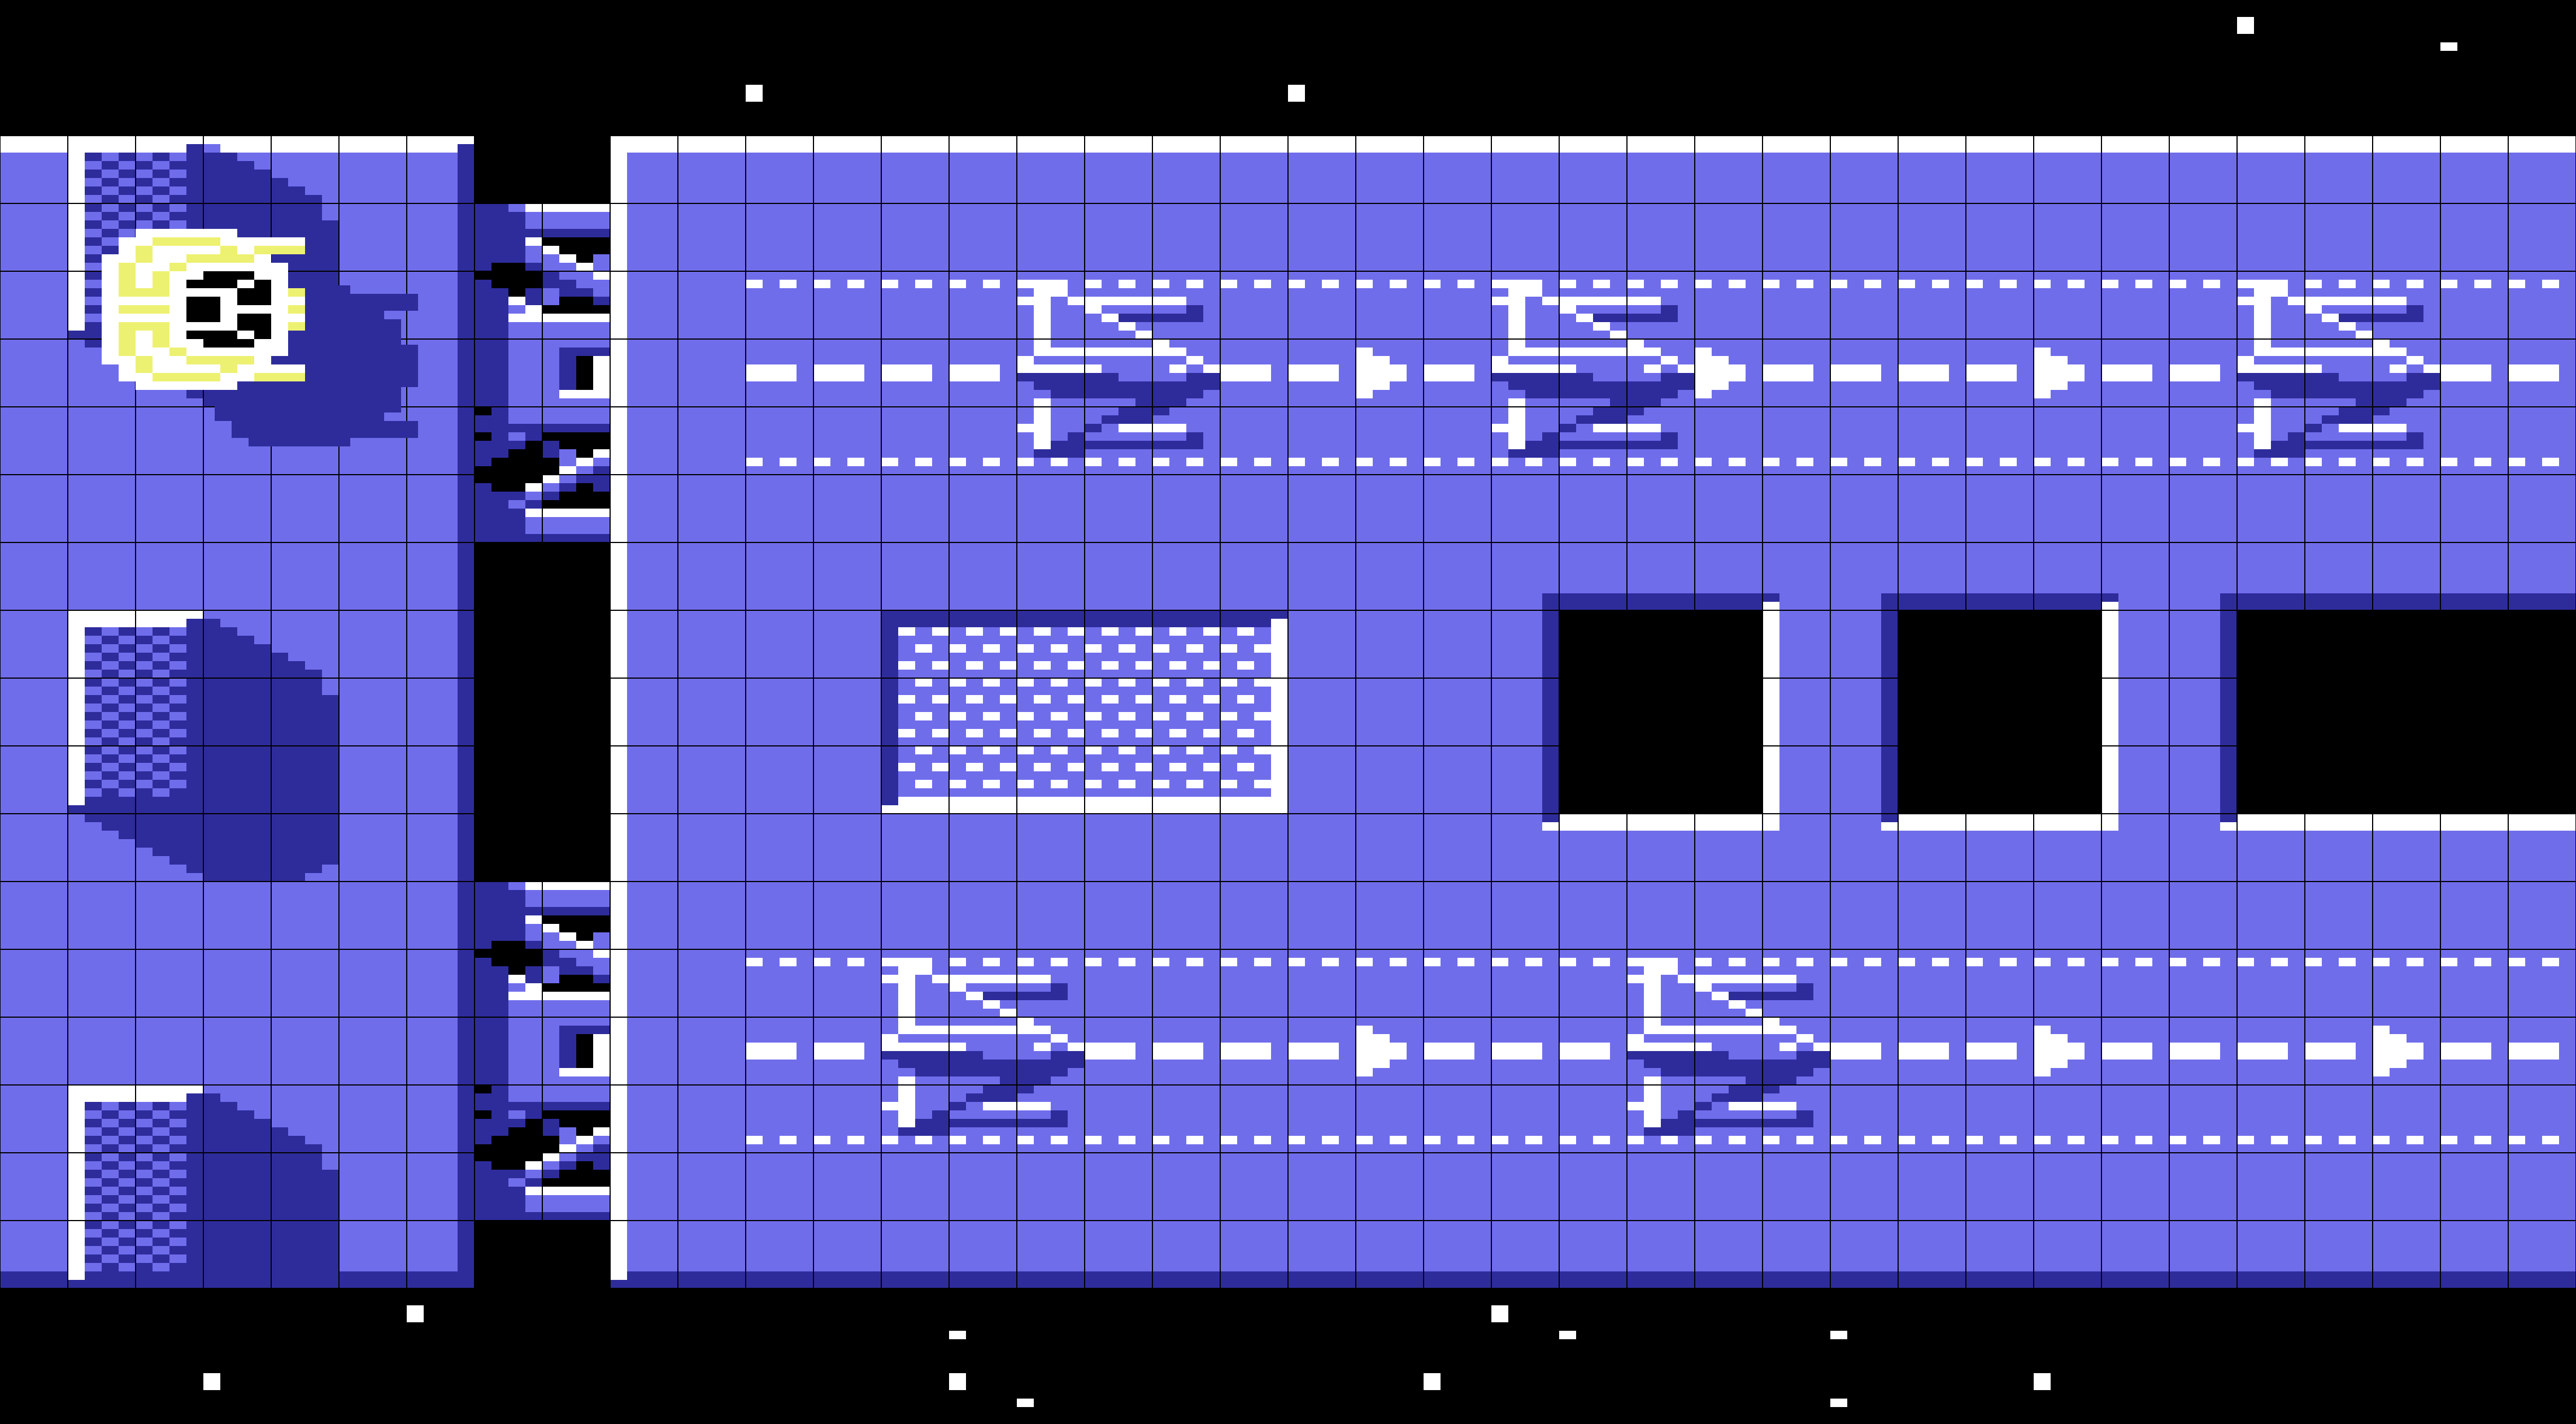
\includegraphics{src/starfield/dreadnought_with_stars_full.png}%
    \end{adjustbox}
\end{figure}
\vspace{-0.4cm}

There is one final twist in \icode{AddStarsBehindDreadnought}. As the dreadnought scrolls
across the screen, one pixel at a time, we will end up with a very unfortunate artefact if
we don't take some remedial action. The sequence below gives you an idea of the problem. As the
segment of the surface in the diagram below moves to the right one pixel at a time, the star moves along with it. 
This is not how the stars should behave at all - they should remain fixed in their position.

\begin{figure}[H]
    \centering
\raisebox{-0.3\totalheight}{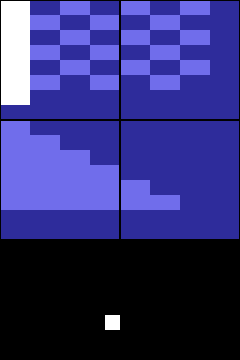
\includegraphics[height=2.0cm]{src/starfield/star_moving_with_dreadnought0.png}}
\hspace{0.1cm}
\raisebox{-0.3\totalheight}{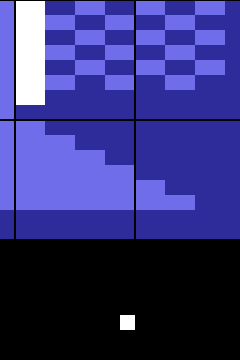
\includegraphics[height=2.0cm]{src/starfield/star_moving_with_dreadnought1.png}}
\hspace{0.1cm}
\raisebox{-0.3\totalheight}{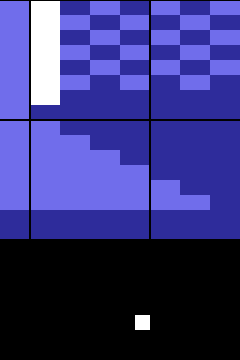
\includegraphics[height=2.0cm]{src/starfield/star_moving_with_dreadnought2.png}}
\hspace{0.1cm}
\raisebox{-0.3\totalheight}{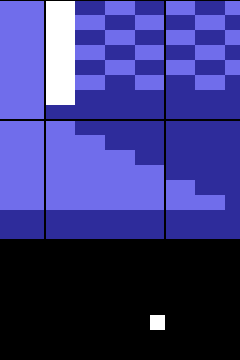
\includegraphics[height=2.0cm]{src/starfield/star_moving_with_dreadnought3.png}}
\hspace{0.1cm}
\raisebox{-0.3\totalheight}{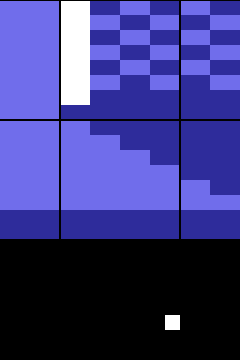
\includegraphics[height=2.0cm]{src/starfield/star_moving_with_dreadnought4.png}}
\hspace{0.1cm}
\raisebox{-0.3\totalheight}{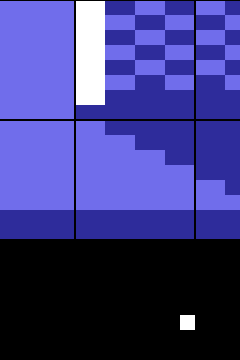
\includegraphics[height=2.0cm]{src/starfield/star_moving_with_dreadnought5.png}}
\hspace{0.1cm}
\raisebox{-0.3\totalheight}{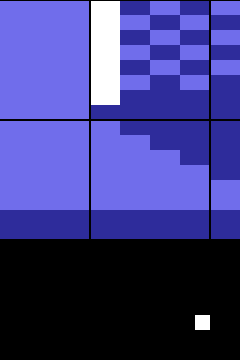
\includegraphics[height=2.0cm]{src/starfield/star_moving_with_dreadnought6.png}}
\hspace{0.1cm}
\raisebox{-0.3\totalheight}{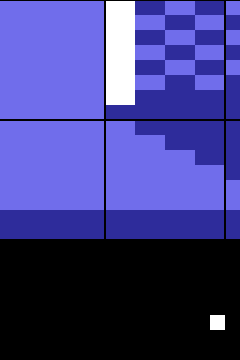
\includegraphics[height=2.0cm]{src/starfield/star_moving_with_dreadnought7.png}}
\end{figure}
\vspace{-0.4cm}

This unintended side-effect is because the hardware feature used to achieve pixel-grained scrolling will move the entire contents of the
screen, including the stars. The end result is that the stars appear to be spinning rapidly in a tight little orbit
as they move from right to left and around again within their single character boundary. Instead of the above, what
we actually want to happen is this.

\begin{figure}[H]
    \centering
\raisebox{-0.3\totalheight}{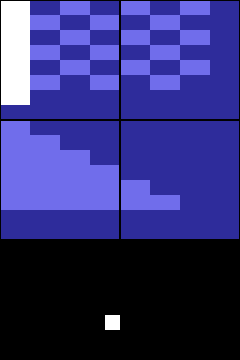
\includegraphics[height=2.0cm]{src/starfield/star_not_moving_with_dreadnought0.png}}
\hspace{0.1cm}
\raisebox{-0.3\totalheight}{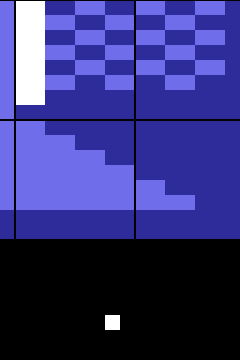
\includegraphics[height=2.0cm]{src/starfield/star_not_moving_with_dreadnought1.png}}
\hspace{0.1cm}
\raisebox{-0.3\totalheight}{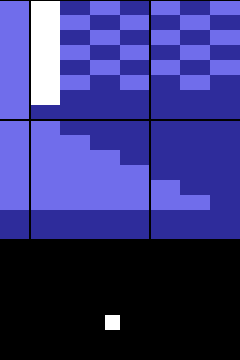
\includegraphics[height=2.0cm]{src/starfield/star_not_moving_with_dreadnought2.png}}
\hspace{0.1cm}
\raisebox{-0.3\totalheight}{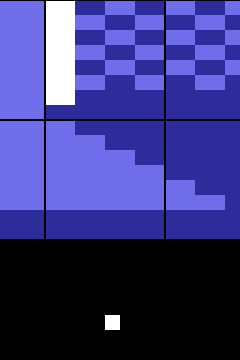
\includegraphics[height=2.0cm]{src/starfield/star_not_moving_with_dreadnought3.png}}
\hspace{0.1cm}
\raisebox{-0.3\totalheight}{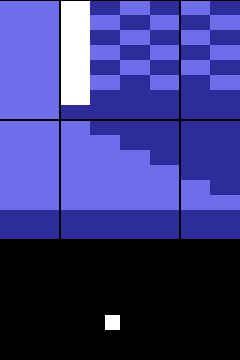
\includegraphics[height=2.0cm]{src/starfield/star_not_moving_with_dreadnought4.png}}
\hspace{0.1cm}
\raisebox{-0.3\totalheight}{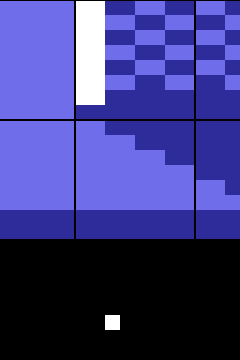
\includegraphics[height=2.0cm]{src/starfield/star_not_moving_with_dreadnought5.png}}
\hspace{0.1cm}
\raisebox{-0.3\totalheight}{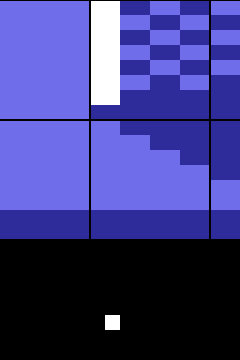
\includegraphics[height=2.0cm]{src/starfield/star_not_moving_with_dreadnought6.png}}
\hspace{0.1cm}
\raisebox{-0.3\totalheight}{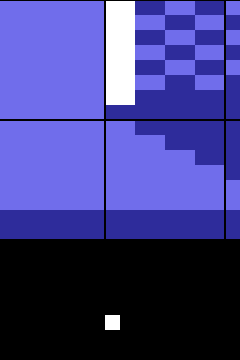
\includegraphics[height=2.0cm]{src/starfield/star_not_moving_with_dreadnought7.png}}
\end{figure}
\vspace{-0.4cm}

While the surface of the dreadnought moves, we keep the star rooted to its spot. The solution that achieves this requirement
is ingenious in its way. What we will do is update the definition of our stars to move the white dot one pixel
to the left for every pixel that the dreadnought will move to the right. We can see two examples of this below.

In the first, we plan to scroll three pixels to the right so we update the star's initial position three pixels to the left.
In the second we will scroll five pixels, so we again update the star with an initial position five pixels to the left. In both cases,
the star ends up in the same position after scrolling, on the extreme right of the character boundary. In other 
words, it will always appear to stay in a fixed position while the surface above it appears to move!

\begin{figure}[H]
    \centering
    \begin{adjustbox}{center}
      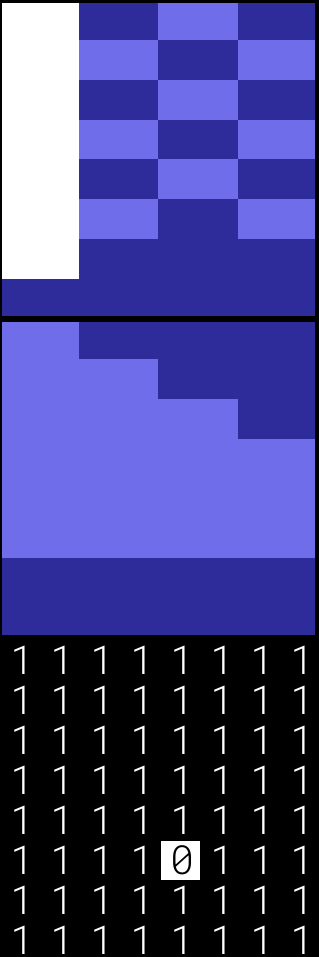
\includegraphics[width=1.0cm]{src/starfield/not_moving_with_dreadnought3_before.png}%
      \hspace{0.5cm}
      \raisebox{1.8\totalheight}{
\includegraphics[height=0.6cm]{src/baydoor_sprites/arrow.png}}
      \hspace{0.3cm}
      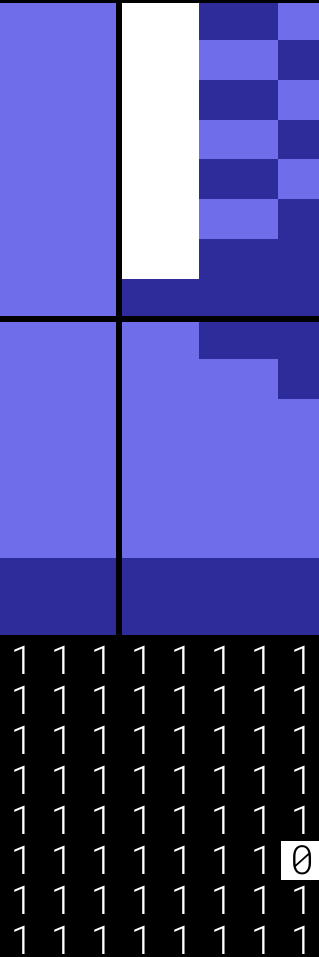
\includegraphics[width=1.0cm]{src/starfield/not_moving_with_dreadnought3_after.png}%
      \hspace{3.2cm}
      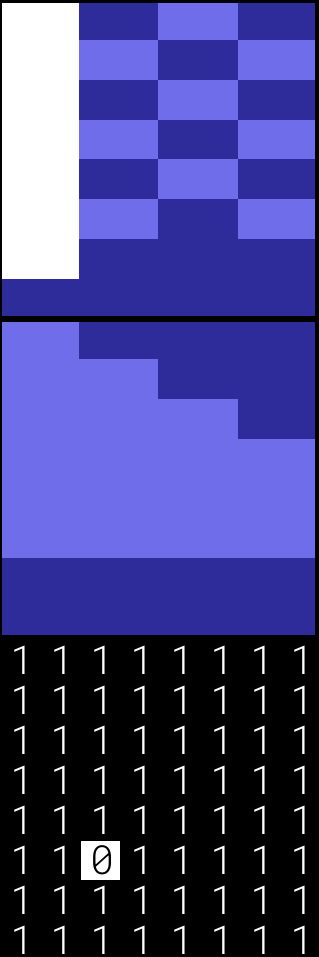
\includegraphics[width=1.0cm]{src/starfield/not_moving_with_dreadnought5_before.png}%
      \hspace{0.5cm}
      \raisebox{1.8\totalheight}{
\includegraphics[height=0.6cm]{src/baydoor_sprites/arrow.png}}
      \hspace{0.3cm}
      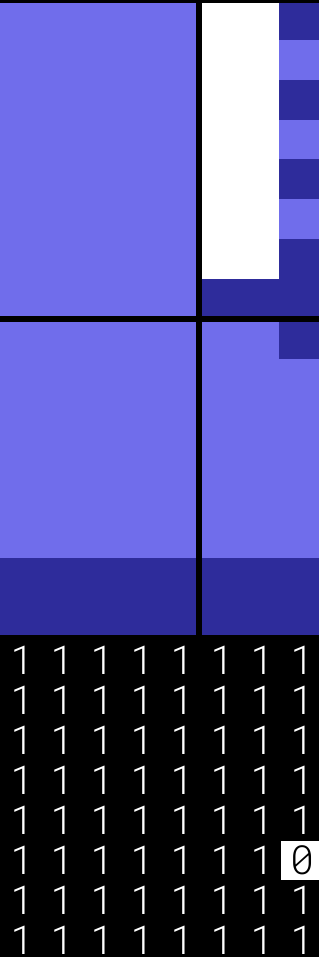
\includegraphics[width=1.0cm]{src/starfield/not_moving_with_dreadnought5_after.png}%
    \end{adjustbox}
\end{figure}
\vspace{-0.4cm}

Armed with this idea we can create an array of the required values for all eight possible scroll values, which we will call
\icode{parallaxOffsetsForStars}.
\begin{lstlisting}
parallaxOffsetsForStars .BYTE $FE,$FD,$FB,$F7,$EF,$DF,$BF,$7F
\end{lstlisting}

We can see the meaning for these values if we visualize them when they are applied to the character
definition of the star below.

\begin{figure}[H]
    \centering
\raisebox{-0.3\totalheight}{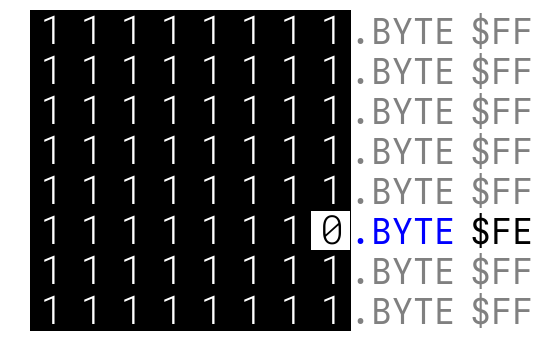
\includegraphics[height=2.1cm]{src/starfield/BASIC_SMALL_STAR_0.png}}
\raisebox{-0.3\totalheight}{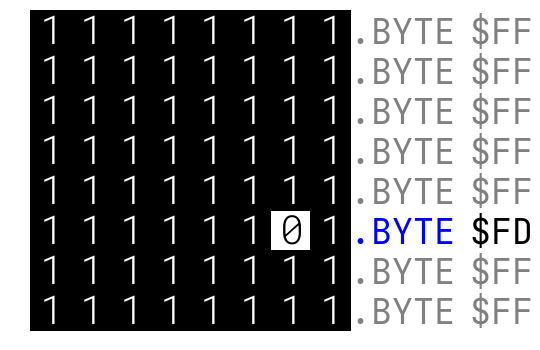
\includegraphics[height=2.1cm]{src/starfield/BASIC_SMALL_STAR_1.png}}
\raisebox{-0.3\totalheight}{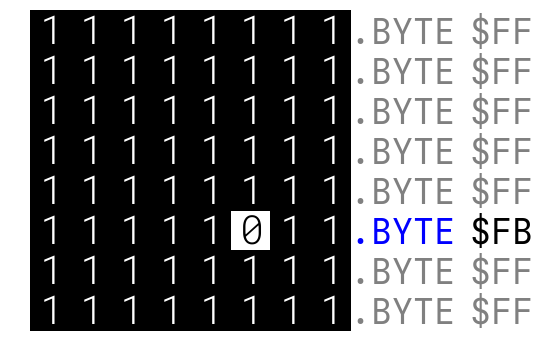
\includegraphics[height=2.1cm]{src/starfield/BASIC_SMALL_STAR_2.png}}
\raisebox{-0.3\totalheight}{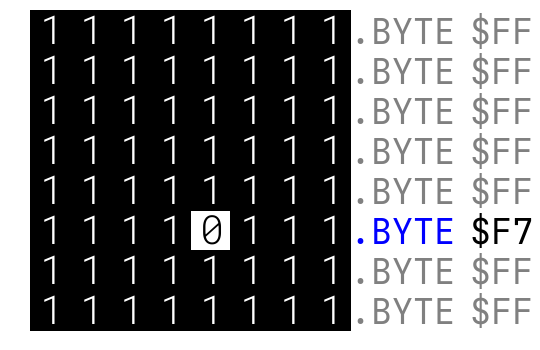
\includegraphics[height=2.1cm]{src/starfield/BASIC_SMALL_STAR_3.png}}
\raisebox{-0.3\totalheight}{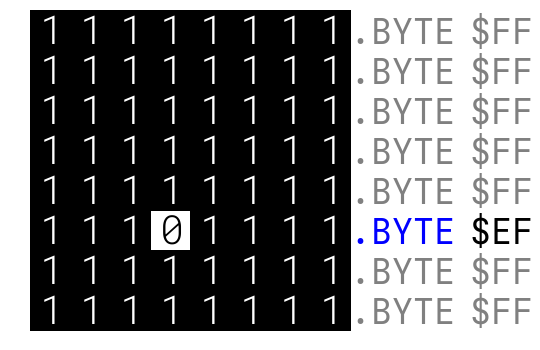
\includegraphics[height=2.1cm]{src/starfield/BASIC_SMALL_STAR_4.png}}
\raisebox{-0.3\totalheight}{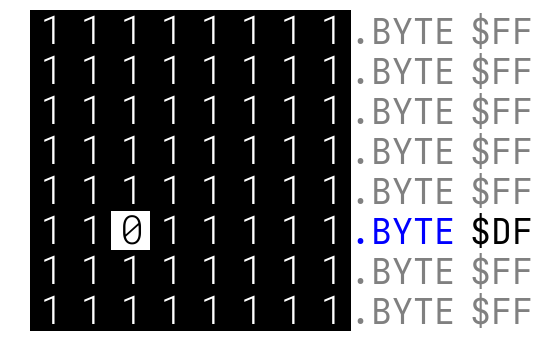
\includegraphics[height=2.1cm]{src/starfield/BASIC_SMALL_STAR_5.png}}
\raisebox{-0.3\totalheight}{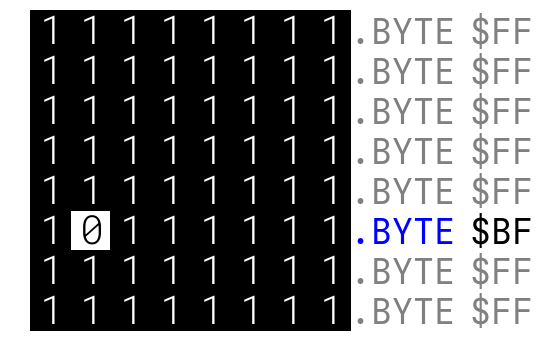
\includegraphics[height=2.1cm]{src/starfield/BASIC_SMALL_STAR_6.png}}
\raisebox{-0.3\totalheight}{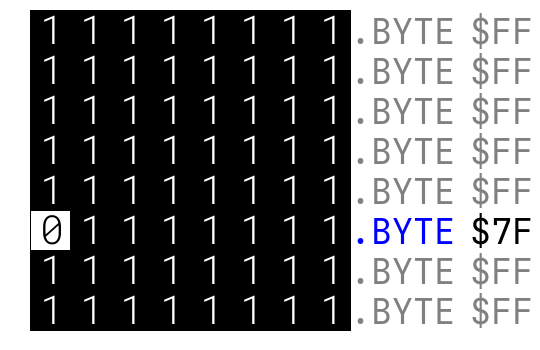
\includegraphics[height=2.1cm]{src/starfield/BASIC_SMALL_STAR_7.png}}
\end{figure}
\vspace{-0.4cm}


With this in hand, all we need is the number of pixels that the C64's hardware will scroll. 
We can then use that number to select a value from this array and write it to the character definition. Notice that the array
is designed in such a way that the number of pixels to scroll will select the appropriate update to
the star. For example, if we are scrolling by five pixels, using \icode{5} as our index
into \icode{parallaxOffsetsForStars} will pick an update for the star that will offset it five pixels to 
the left.

The code below performs this relatively straightforward task, updating the byte in the character definition to move the position of the star according to the
value in \icode{pixelsToScroll}. (We will see how the value in \icode{pixelsToScroll} is calculated in the next chapter).
\begin{lstlisting}
  LDX pixelsToScroll            ; Load pixels to scroll to X.
  LDA parallaxOffsetsForStars,X ; Use it to select our value. 
  STA smallStarXPosition        ; Update the character definition.
\end{lstlisting}

This will have the desired effect for the small star: moving it to the left the desired number of pixels
before it is ultimately moved back into its 'fixed' position after scrolling. Notice that if the number of
pixels to scroll is 'zero', i.e. we are not performing any pixel-grained scrolling at all, we will select the first
element in the \icode{pixelsToScroll} array, which is the default, desired position of the star on the extreme
right of the character boundary.

To perform the same effect for the larger star it is just a question of applying the same updates at the appropriate positions in the definition.

\begin{lstlisting}
  STA bigStarTopXPosition      ; Update the big star character definition.
  STA bigStarBottomXPosition   ; Update the big star character definition.
\end{lstlisting}

Again, we can visualize these updates below. The values and the method are the same, we just repeat them
to create an elongated star consisting of two stacked pixels.

\begin{figure}[H]
    \centering
\raisebox{-0.3\totalheight}{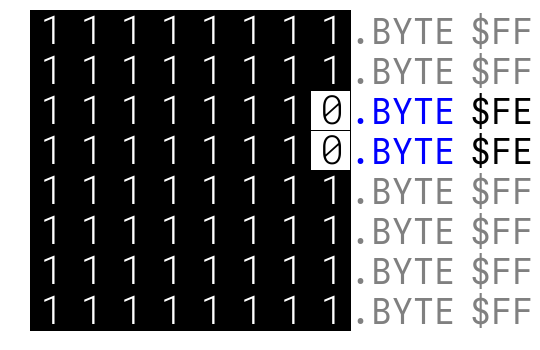
\includegraphics[height=2.1cm]{src/starfield/BASIC_BIG_STAR_0.png}}
\raisebox{-0.3\totalheight}{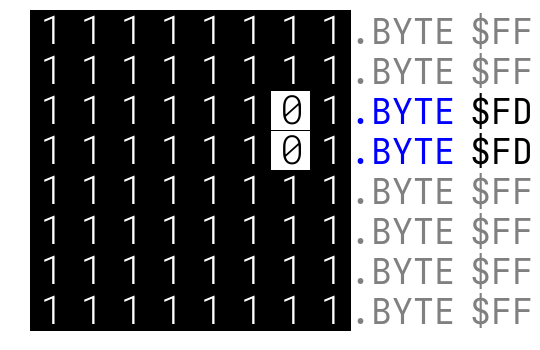
\includegraphics[height=2.1cm]{src/starfield/BASIC_BIG_STAR_1.png}}
\raisebox{-0.3\totalheight}{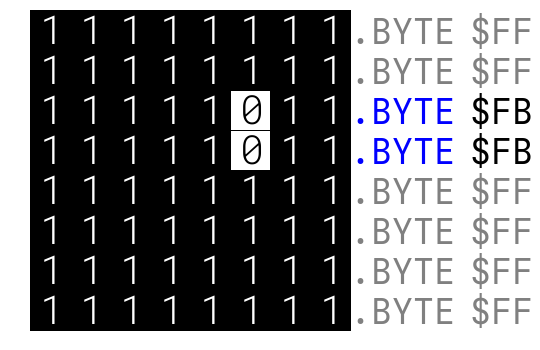
\includegraphics[height=2.1cm]{src/starfield/BASIC_BIG_STAR_2.png}}
\raisebox{-0.3\totalheight}{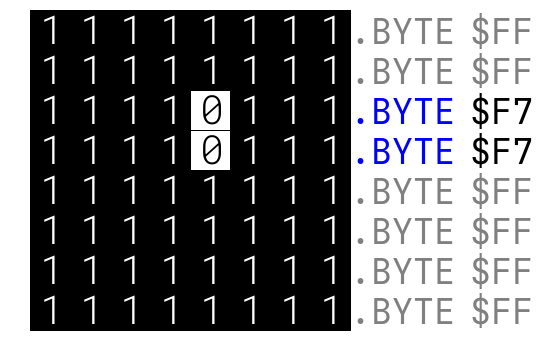
\includegraphics[height=2.1cm]{src/starfield/BASIC_BIG_STAR_3.png}}
\raisebox{-0.3\totalheight}{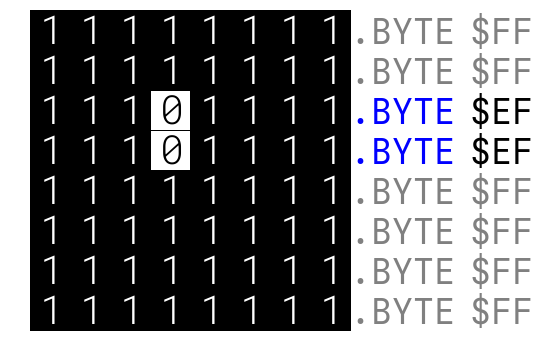
\includegraphics[height=2.1cm]{src/starfield/BASIC_BIG_STAR_4.png}}
\raisebox{-0.3\totalheight}{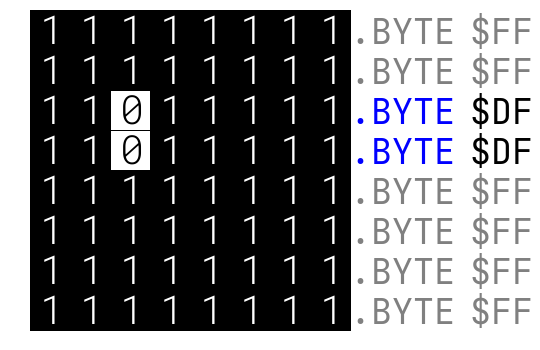
\includegraphics[height=2.1cm]{src/starfield/BASIC_BIG_STAR_5.png}}
\raisebox{-0.3\totalheight}{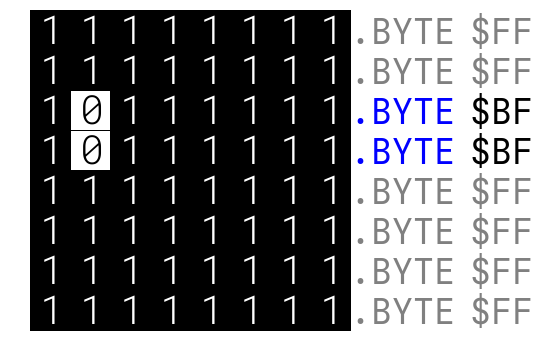
\includegraphics[height=2.1cm]{src/starfield/BASIC_BIG_STAR_6.png}}
\raisebox{-0.3\totalheight}{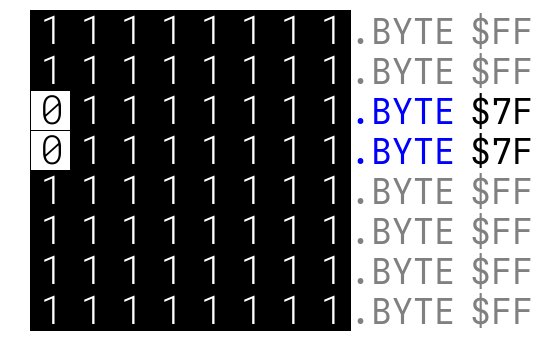
\includegraphics[height=2.1cm]{src/starfield/BASIC_BIG_STAR_7.png}}
\end{figure}
\vspace{-0.4cm}

